% !TEX root = ../manuscript.tex
\section{Introduction}

Knowledge-intensive information systems increasingly expose intermediate artifacts during retrieval, annotation, validation, update, and reuse. These artifacts include graph nodes, entity bindings, verification records, rule-like operations, retrieval checks, process annotations, and reasoning traces. Once exposed, they become knowledge artifacts that must be represented, organized, curated, and reused across the knowledge lifecycle. The challenge is that these artifacts are heterogeneous, uncertain, and often more numerous than the audit capacity available to curators.

Existing methods supply useful fields for this setting. Process-annotation methods attach scalar quality estimates to intermediate artifacts. Local utility methods estimate artifact influence. Graph-based salience methods identify structurally prominent nodes. Fixed-budget audit also needs a reusable record that combines these fields with dependency structure and audit interpretation. Such a record helps curators see whether an artifact provides local evidence, supports a dependency, duplicates earlier support, or exposes a downstream bottleneck.

This paper introduces Structurally-Calibrated Functional Metacognitive Attribution (SC-FMA) as a knowledge representation transformation layer for this setting. In SC-FMA, ``metacognitive'' is used operationally. It names engineered secondary inspection of observable attribution-related artifacts through structural and functional decomposition; it is not a claim about latent cognitive-state monitoring. Readers can equivalently read the method as structurally calibrated functional attribution over observable process artifacts. SC-FMA transforms intermediate knowledge artifacts into structured audit records that represent dependencies, calibrate supplied annotation or utility fields, attach audit reasons and interpretations, and treat audit priority as one field within the record.

SC-FMA organizes fixed-budget audit around a structured record. Process-annotation studies provide artifact-level fidelity fields~\cite{lightman2023verify,uesato2022solving}. Network and graph-explanation methods show why structural position, redundancy, and bottleneck exposure can matter~\cite{albert2000error,newman2010networks,ying2019gnnexplainer}. Simplex projection provides a familiar way to impose a fixed review budget~\cite{wang2013projection}. SC-FMA combines these ingredients as record fields: fidelity, structure, redundancy, bottleneck protection, and budget consistency.

The paper makes three contributions. First, it formulates fixed-budget audit-record construction for structured knowledge artifacts. Second, it introduces SC-FMA and the SCU objective, which combine fidelity fields, structural dependency, redundancy, and bottleneck roles into decomposed audit records. Third, it evaluates the representation on a PRM800K process-annotation dataset, a Countries-KG backend feasibility study, rule-derived audit-target retrieval, and controlled synthetic calibration.

The main findings follow the same knowledge-engineering workflow, with a negative result at the center of the real-data route. On the PRM800K process-annotation dataset, \wstruct{} is treated as a supervised fidelity field for artifact records and remains the strongest real-data ranking field. Under the frozen hash split (4,417 samples and 34,219 labeled artifacts), SC-FMA Ridge closely tracks \wstruct{} (Spearman $\rho = 0.604$ versus $0.611$) while exposing decomposition fields; QP and Projection are lower-consistency variants on this strong-fidelity route, and QP degrades most strongly on long traces. The Countries-KG backend feasibility study shows that typed ontology edges can change structural-dependency representation at the graph interface, but this sensitivity is also a reliability warning for the structural-necessity signal. Rule-derived audit-target retrieval provides a field-level readout of weak utility anchors, redundancy, and structural over-correction, plus a QP-derived bottleneck consistency check; a raw-field control separates field exposure from SCU joint optimization. Controlled synthetic calibration and ablation explain implementation behavior when labels explicitly encode structural preferences, not external audit value.

The remainder of this paper is organized as follows. Section~\ref{sec:related-work} reviews attribution, step-level annotation signals, graph-based knowledge engineering, and audit methods. Section~\ref{sec:methods} presents SC-FMA, the SCU objective, and its representation properties. Section~\ref{sec:experimental-results} reports evidence from real annotation data, knowledge-graph backend feasibility, and controlled calibration. Section~\ref{sec:discussion} interprets the method in the knowledge lifecycle. Section~\ref{sec:conclusions} concludes.

Figure~\ref{fig:overall-framework} gives the high-level knowledge-engineering workflow. SC-FMA sits between raw knowledge artifacts and potential review workflows: it represents artifacts as dependency graphs, calibrates annotation signals with SCU, and returns knowledge audit records with explicit structural roles and interpretations.

\begin{figure}[pos=ht]
\centering
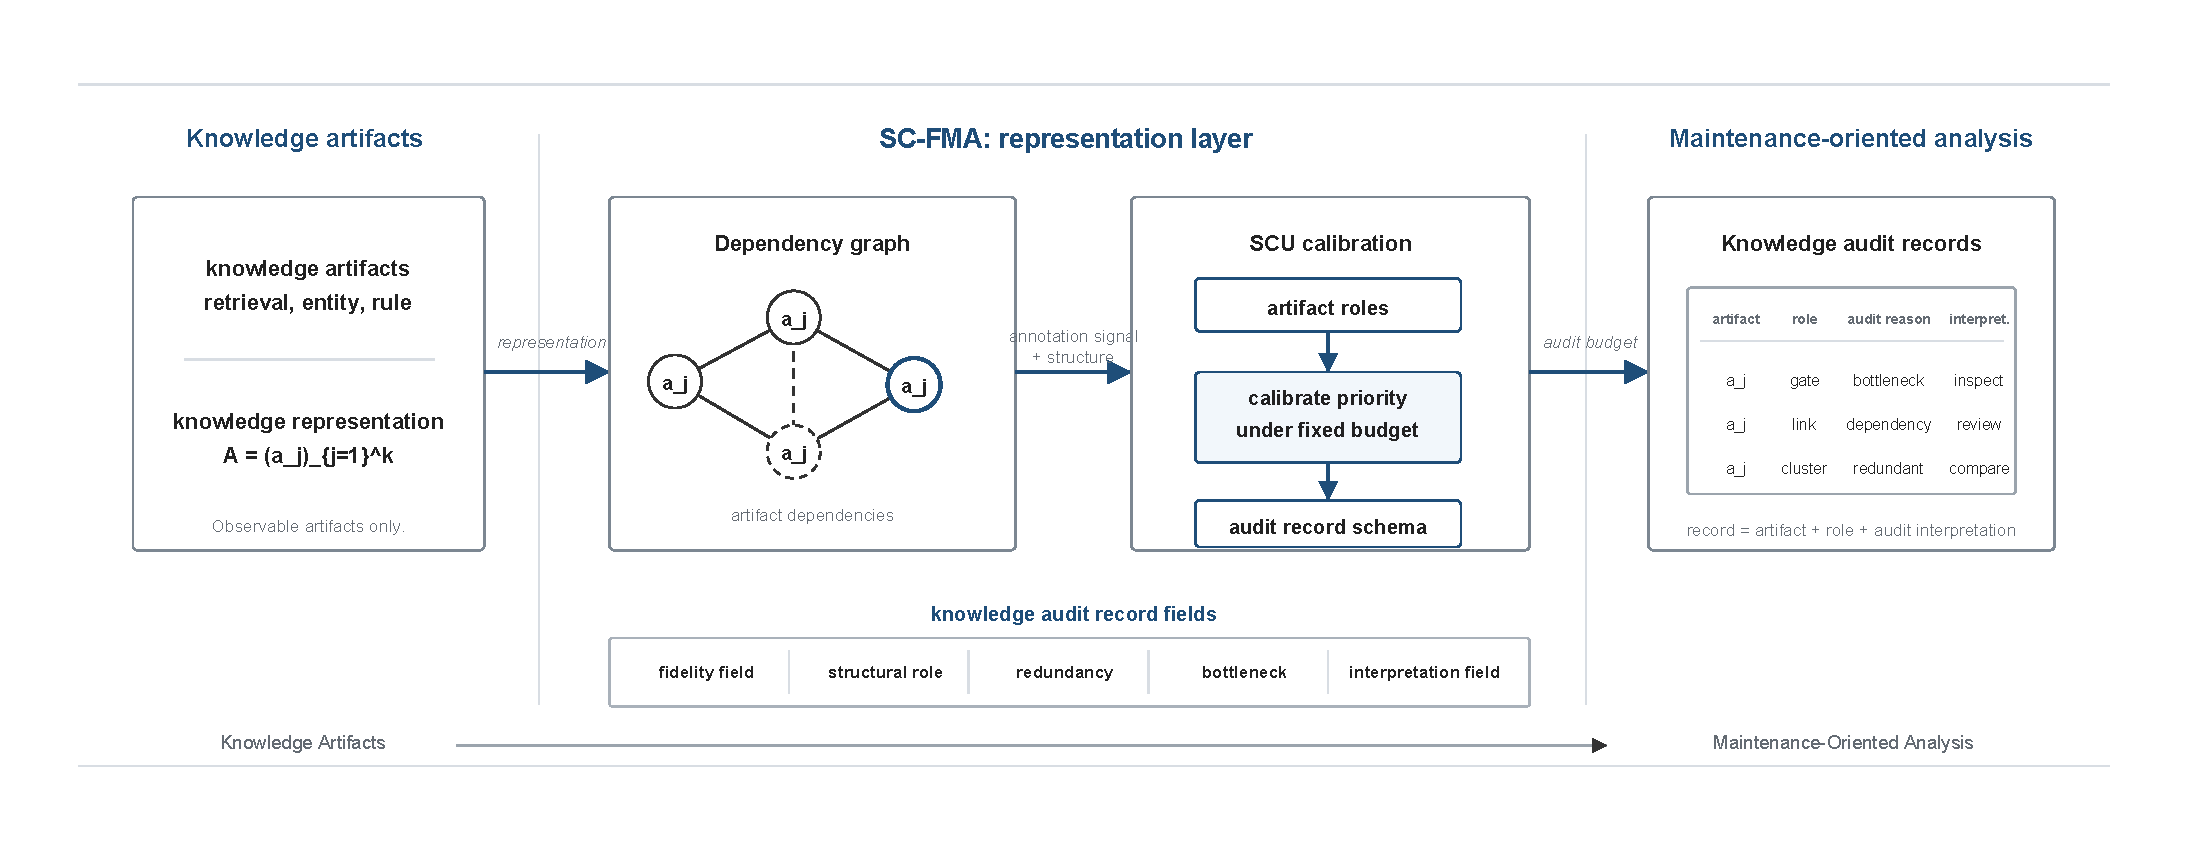
\includegraphics[width=\linewidth]{figures/fig_overall_framework.pdf}
\caption{Knowledge engineering workflow for SC-FMA. The figure should be read as a transformation from Knowledge Artifact $\rightarrow$ Representation $\rightarrow$ Graph Structure $\rightarrow$ SCU $\rightarrow$ Audit Record $\rightarrow$ Knowledge Curation. Raw reasoning traces, graph nodes, and process annotations are first organized as auditable knowledge artifacts, then represented through dependency-aware graph structure. SCU constructs structured audit records by preserving annotation or utility fidelity while adding structural dependency, redundancy, bottleneck, audit-reason, and interpretation fields. The resulting records support fixed-budget audit representation and analysis; the audit-priority field is only a downstream use of the audit representation.}
\label{fig:overall-framework}
\end{figure}

